\chapter{Literature Review}
\section{Service System Engineering}
Service engineering is a topic that is being discussed in today's technological world. Various forms of information technology development has now led to the service (services). It is also the underlying desire of the writer to lift a research thesis that incorporates service engineering to produce a good disaster management.\par

\subsection{Services}
\label{sebsec: ServicesDefinition}
Services are activities that cause a transformation of the state of an entity (people, product, business, and region or nation) by mutually agreed terms between the service provider and the customer. Individual services are relatively simple, although they may require customization and significant backstage support (e.g., database, knowledge management, analysis, forecasting, etc.) to assure quality and timely delivery. \par
Many term used in service science to describe service system. In this research, we choose to use Service System Engineering(SSE) term in order to not make confuse. Service System Engineering is a multidisciplinary approach to manage and design value co-creation of a service system. It extends the holistic view of a system to a customer-centric, end-to-end view of service system design \cite{SSEDefinition}. In other meaning, the approaches define to engineer system of system that are linked together so that can improve robustness, lower cost and increase liability. \par
\begin{comment}
	servvis adalah segala bentuk aktivitas yang mengtranformasi atau meubah bentuk dari sebuah entitas seperti masyarakat, procukatau bisnis dengan sebuah bentuk kepercayaan bersama antara si penyedia service atu layanan dengan si kostumer.
	
	sedangkan rekayasa sistem layanan adalah pendekatan-pendekatan yang yang diberikan untuk mengatur atau mendesain sebuah nilai dari sebuah sistem layanan. atau boleh dikatakan sebuah pendekatan untuk merekayasa sebuah sistem layanan untuk mendepatkan  tingkat ketahanan sistem yang lebih baik, mengurangi biaya dan meningkatkan kekuatan sistem.
	
	liability artinya bertanggung jawab, kecenderungan atau kekurangan
\end{comment}

Service System Engineering (SSE) has two core concept. Lopez and Pineda (2013) mention two core concept of SSE are service Meta-Model and Service Systems Development Process (SSDP). Service meta-model comprised of nine types of system entities to help business challenge and to create the the service value chain among relevant stakeholders to co-create the value.\par
\begin{table}[H] 
\begin{center}
\caption{Service Meta Model}
\label{tab: TabelServiceMeta}
	\vspace{0.1cm}
\begin{tabular}{ |p{3cm}|p{9cm}| }
 \hline
 \textbf{Entity} & \textbf{Atributes}\\
 \hline \hline
 Customers & Features, attitudes, preferences, requirements \\
 \hline 
 Goals & Business, service, customer\\
 \hline
 Inputs & Physical, information, knowledge, constraint\\
 \hline
 Output & Physical, information, knowledge, waste, customer satisfaction\\
 \hline
 Process & Service provision, service delivery, service operation, service support, customer relationship, planning and control\\
 \hline
 Human Enablers & Service providers, support providers, management, owners organization, customers\\
 \hline
 Physical enablers & Enterprise, building, equipment, enabling technologies, furnishing, etc\\
 \hline
 Informatics Enablers & information, knowledge, methods, process and tools (MPTs), decision support, skill acquisition. \\
 \hline
 Environment &Political, economic, social, technological, environmental factors.\\ 
 \hline
\end{tabular}
\end{center}
\end{table}\par

Next step after defining the entities needed in the system is building the process. The process built should have concern to tier of services entities to realize the overall service system. Lopez and Pineda (2013) purposed The Service Systems Development Process (SSDP) develop the service. SSDP consists of several repeating life-cycle phases with required inputs and expected outputs for each phase to help understand the activities required for realizing service systems. The system engineering phases are evolved to adapt and improve systems engineering methodologies to address the nature of Service Systems. The figure \ref{fig:SSDP} will offered a model of SSDP.\par

\begin{figure}[H]
    \begin{center}
    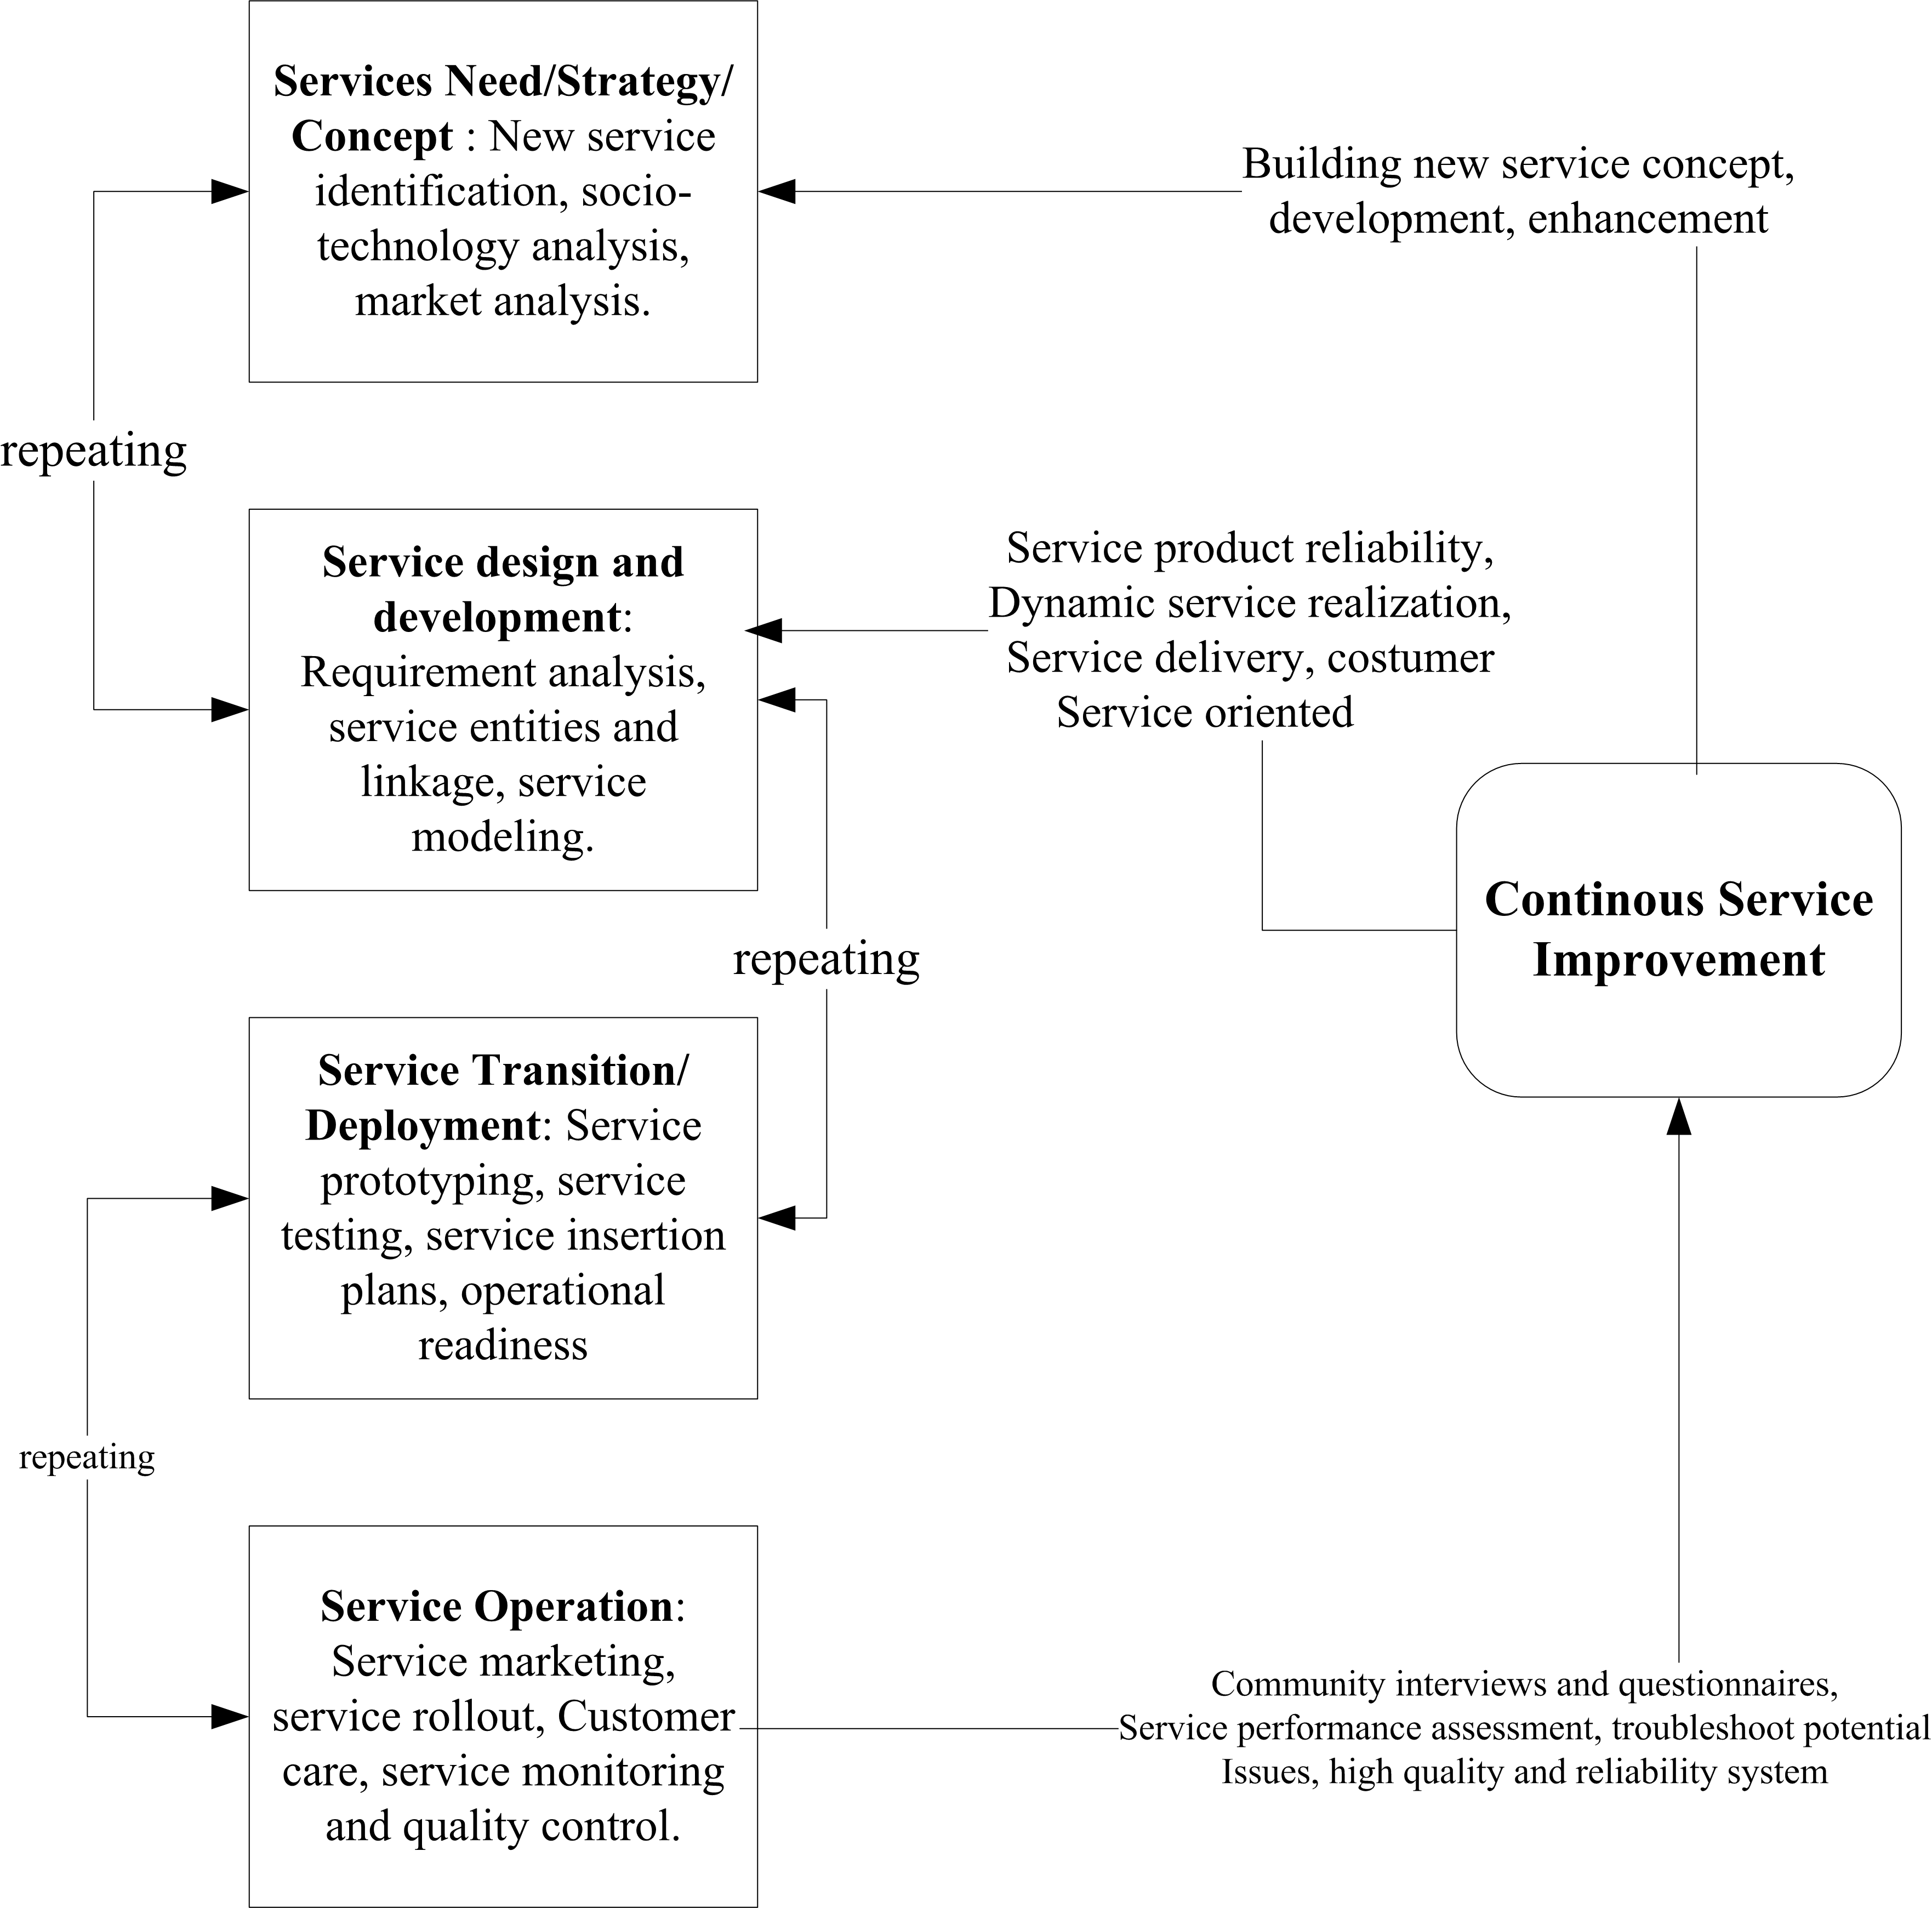
\includegraphics[scale=0.7]{sed.png}
        \caption{Service System Development Project\cite{Lopes2013}}
        \label{fig:SSDP}
    \end{center}
\end{figure}

The SSDP will identify the required input activities that execute to discover and designing the potential service needed and help analyze the service systems from an end-to-end perspective. During the service strategy phase new services are identified based on end user needs, mass collaboration trends, technology trends, and/or government/organization strategies. The government or stakeholder can decides to pursue the development of the selected service systems based on an extensive socio-techno-economic feasibility study. Service Life Cycle Management (LCM) methodologies such as continuous service improvement are utilized to analyze and set service improvements, potential service enhancements and to identify new service concepts across all entity types. Service LCM also includes strategies for replacement or disposal of the service/service entities, if applicable.\par

\subsection{Service Oriented Architecture}
The term service is widely used in the context of business and information technology. It is commonly understood as a facility supplying some public demand\cite{Haubrock2007}. This implies that a service can be performed by different entities, i.e. a human being, an enterprise as well as a hardware or software device as long as the idea of a service consumer on the one and a service provider on the other side is valid.\par
A service is a provider/client interaction that creates and captures value\cite{Haubrock2007}. The term SOA refers to service creation, interaction, presentation, and integration infrastructure capabilities to build business-level software based on reusable components. While this definition originates from Information Technology, it refers to several different aspects and disciplines involved in this approach: business processes, design and usability. In another meaning, SOA is essentially a collection of services. These services communicate with each other. The communication can involve either simple data passing or it could involve two or more services coordinating some activity. Some means of connecting services to each other is needed\cite{DefinisiSOA}.\par

\begin{figure}[H]
\centering
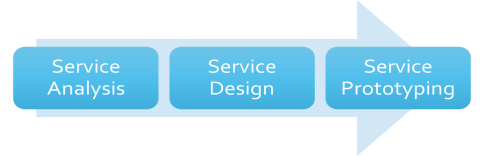
\includegraphics[scale=0.7]{ServiceEgineeringFramework.png}
	\caption{Service Engineering Framework}
	\label{fig:SEFramework}
\end{figure}

%% paragraph di bawah masih perlu perbaikan, karena full copy paste 
The new layer of abstraction introduced with service orientation now bares the potential to bridge the communication gap between IT developers and experts using these services, introducing a new business process- driven approach. For disaster management, this separation of concerns between definition and description of business processes and its actual implementation in form of computational services bares the potential to give consideration to the functional heterogeneity of partners involved. Public authorities or other institutions in disaster management are able to under- stand the semantics of the services and can therefore integrate them in their decision making process, while scientists and technicians provide and administrate these components.
SOA\par 

\subsection{Web Services}
Many of the benefits offered by the web service, especially high interoperability and the use that can be accessed anytime and anywhere as long as connected to the Internet network. Web service based on web standards and XML. web services discount significant role in SOA. Web services built upon protocols that already exist and have a platform independent, such as HTTP, XML, UDDI and WSDL. Those protocols provide services that can be found and used dynamically. SOA provides a service that has a contract that is platform independent interface, provided by XML. SOA emphasis on interoperability, it is provided by HTTP. This is what makes web services as the backbone of SOA.\par

\subsection{Unified Modeling Language}
Modeling is the designing of software applications before coding. Modeling is an Essential Part of large software projects, and helpful to medium and even small projects as well\cite{DefinisiUML}. A model plays the analogous role in software development that blueprints and other plans (site maps, elevations, physical models) play in the building of a skyscraper. Using a model, those responsible for a software development project's success can assure themselves that business functionality is complete and correct, end-user needs are met, and program design supports requirements for scalability, robustness, security, extendibility, and other characteristics, before implementation in code renders changes difficult and expensive to make. Surveys show that large software projects have a huge probability of failure - in fact, it's more likely that a large software application will fail to meet all of its requirements on time and on budget than that it will succeed\cite{DefinisiUML}.\par
UML 2.0 defines thirteen types of diagrams, divided into three categories, Six diagram types represent static application structure, three represent general types of behavior and four represent different aspects of interactions,
\begin{enumerate}
\setlength{\itemsep}{1.5pt}
\setlength{\parskip}{1.5pt}
\item [1.]\textbf{Structure Diagrams} include the Class Diagram, Object Diagram, Component Diagram, Composite Structure Diagram, Package Diagram, and Deployment Diagram. 
\item [2.]\textbf{Behavior Diagrams} include the Use Case Diagram (used by some methodologies during requirements gathering); Activity Diagram, and State Machine Diagram.
\item [3.]\textbf{Interaction Diagrams}, all derived from the more general Behavior Diagram, include the Sequence Diagram, Communication Diagram, Timing Diagram, and Interaction Overview Diagram.
\end{enumerate}
\begin{figure}[H]
    \begin{center}
    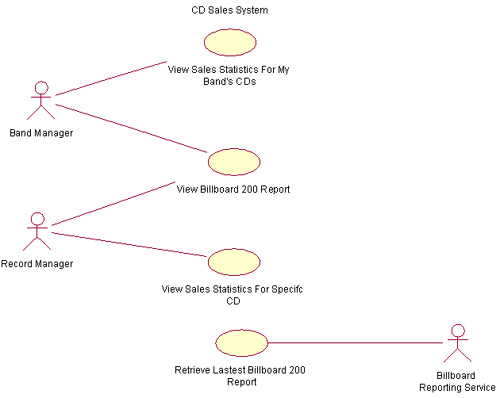
\includegraphics[scale=0.4]{contohUML.jpg}
        \caption{Sample of Use-Case Diagram \cite{SampleOfSimpleUML}}
        \label{fig:use-caseDiagram}
    \end{center}
\end{figure}

\subsection{Geographic Information System}
A geographic information system (GIS) is a computer system for capturing, storing, checking, and displaying data related to positions on Earth’s surface\cite{DefiniGIS}. GIS can show many different kinds of data on one map. This enables people to more easily see, analyze, and understand patterns and relationships. With GIS technology, people can compare the locations of different things in order to discover how they relate to each other. For example, using GIS, the same map could include sites that produce pollution, such as gas stations, and sites that are sensitive to pollution, such as wetlands. Such a map would help people determine which wetlands are most at risk.\par 

GIS can use any information that includes location. The location can be expressed in many different ways, such as latitude and longitude, address, or ZIP code. Many different types of information can be compared and contrasted using GIS. The system can include data about people, such as population, income, or education level (\figurename{\ref{fig:DefinisiGIS}}). It can include information about the land, such as the location of streams, different kinds of vegetation, and different kinds of soil. It can include information about the sites of factories, farms, and schools, or storm drains, roads, and electric power lines.\par
\begin{figure}[H]
    \begin{center}
    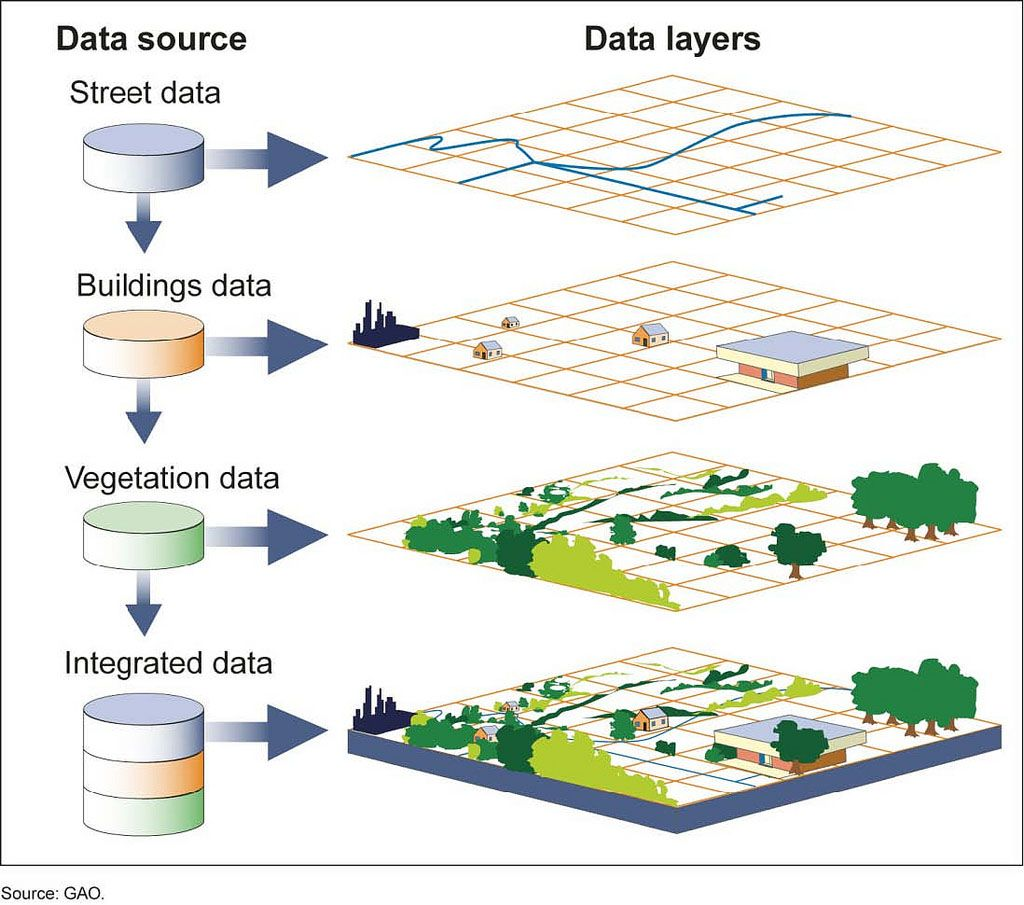
\includegraphics[scale=0.3]{gis.jpg}
        \caption{Multiple Layers of GIS \cite{DefiniGIS}}
        \label{fig:DefinisiGIS}
    \end{center}
\end{figure}\par
\vspace{-1cm}
\subsubsection{Global Positioning System}
The Global Positioning System (GPS) is a satellite-based navigation system made up of a network of 24 satellites placed into orbit by the U.S. Department of Defense\cite{DefiniGPS}. GPS was originally intended for military applications, but in the 1980s, the government made the system available for civilian use. GPS works in any weather conditions, anywhere in the world, 24 hours a day. There are no subscription fees or setup charges to use GPS.\par
GPS satellites circle the earth twice a day in a very precise orbit and transmit signal information to earth. GPS receivers take this information and use trilateration to calculate the user's exact location. Essentially, the GPS receiver compares the time a signal was transmitted by a satellite with the time it was received. The time difference tells the GPS receiver how far away the satellite is. Now, with distance measurements from a few more satellites, the receiver can determine the user's position and display it on the unit's electronic map. A GPS receiver must be locked on to the signal of at least 3 satellites to calculate a 2-D position (latitude and longitude) and track movement. With four or more satellites in view, the receiver can determine the user's 3-D position (latitude, longitude and altitude). Once the user's position has been determined, the GPS unit can calculate other information, such as speed, bearing, track, trip distance, distance to destination, sunrise and sunset time and more.\par 


\subsubsection{Location Based Services}
Location based services (LBS) are services offered through a mobile phone and take into account the device’s geographical location\cite{DefiniLBS}. LBS typically provide information or entertainment. Because LBS are largely dependent on the mobile user’s location, the primary objective of the service provider’s system is to determine where the user is. There are many techniques to achieve this.\par 

Some of the most common LBS applications include local news, directions, points of interest, directory assistance, fleet management, emergency, asset tracking, location-sensitive building, and local advertisement.\par

\subsection{Internet of Things(IoT}
Internet of Things [IoT] is a prevalent technology that is being emerged in information technology today. Since 1991 when IoT was proposed by Kevin Ashton, several research works are carried out in the field of IoT and its relevant technologies. Internet of (IoT) is an integrated part of Future Internet and could be defined as dynamic global network infrastructure with self configuring capabilities based on standard and interoperable communication protocols where physical and virtual "things" have identities, physical attributes and virtual personalities and use intelligent interface and are seamlessly integrated into the information network\cite{IoTDefinition}.

\section{Disaster and Disaster Management}
\vspace{-0.5cm}
\subsection{Disaster}
The term disaster was defined in many definition, there are :
\begin{enumerate}
\item[1.] a serious disruption of the functioning of society, causing widespread human, material and enviromental losses which exceed the ability of affected society to cope using only its own resources\cite{EffisientDM}
\item[2.] an incident or series of incidents that threaten and disrupt the lives and livelihood caused by natural factors and/or non natural factors effected in human casualties, environmental damage loss property and psychological impact\cite{DefinisiBencanaBNPB}.
\item[3.] a severe disruption, ecological and psychosocial, which greatly exceed the coping capacity of the affected community\cite{DisasterDefinition}.
\end{enumerate} \par
\begin{figure}[H]
    \begin{center}
    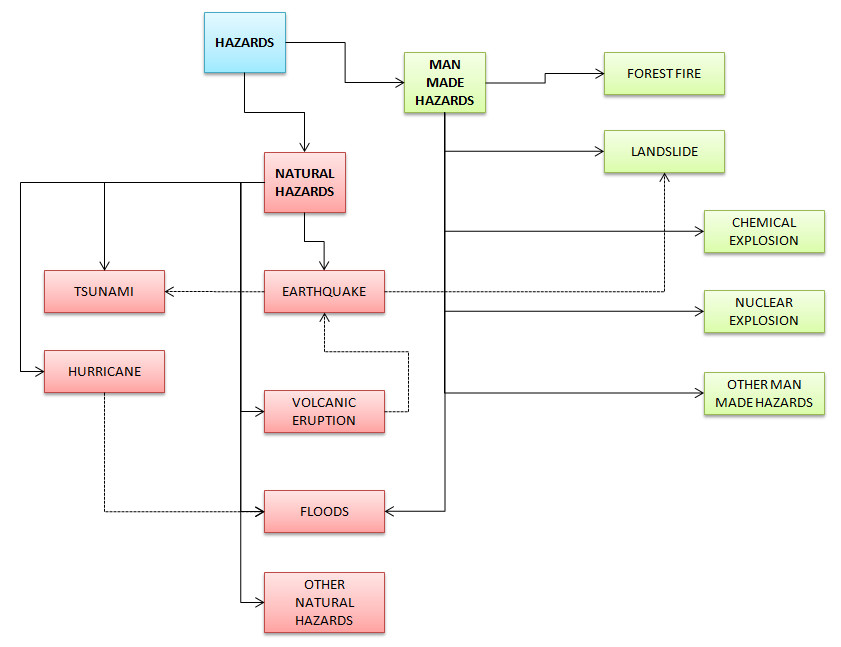
\includegraphics[scale=0.5]{hazardBagan.jpg}
        \caption{Classification of hazard based on causes\cite{definisiHazard}}
        \label{fig:DefinisiHazard}
    \end{center}
\end{figure}
Every community has some coping resources to deal with accidents and emergencies. Coping resources are the individual and community skills, materials, equipment or services that can be used to meet the demands created by an incident. The health care sector forms an important part of this, from the self-administered treatments available at a pharmacy or a walk-in clinic, through the Emergency Medical Services and hospital emergency departments, to the special care provided by burn wards or other tertiary services\cite{DMModelGuideline}.\par
Disaster management aims to shift the threshold at which an impact becomes a disaster\cite{DMModelGuideline}. This is achieved through two main methods: decreasing the amount of damage an impact can cause and increasing the capability of the community?s coping resources to deal with any damage that does occur. Disaster management ensures a coordinated response to make the best use of the community?s coping resources. The long-term recovery of the community is also a basic part of disaster management.\par

Disaster management has become a very important area worth exploration in the last few years, primarily due to the large number of disasters occurring across the world. Disaster management involves coordinating a large number of emergency responders to rescue people and recover infrastructure. The environment in which the responders act is often hazardous and full of uncertainties. Disaster response requirements are often identified by several distinctive characteristics and factors relevant to managing them \cite{MASDIsaster} such as: 
\begin{enumerate}
\setlength{\itemsep}{1.5pt}
\setlength{\parskip}{1.5pt}
\item[1.]disaster overwhelms the available resources 
\item[2.]disaster response should be immediate,
\item[3.]disaster events are unpredictable
\item[4.]uncertainty and incompleteness of information and resources
\item[5.]need for information and communication, and
\item[6.]disaster recovery strategy to recover from secondary crisis. 
\end{enumerate}\par

\subsection{Disaster Management Framework}
Hyogo Framework for Action is a global blueprint for disaster reduction. HFA starts in January 2005 at the world conference on disaster reduction held in Kobe, Hyogo, Japan. The framework is a foundation to 10-year plan to make the world safer from natural hazard. HFA has five priorities, there are\cite{HFAConference}:
\begin{enumerate}
\setlength{\itemsep}{1.5pt}
\setlength{\parskip}{1.5pt}
\item[1.]Ensure that disaster risk reduction is a national and a local priority with a strong institutional basis for implementation.
\item[2.]Identify, assess and monitor disaster risks and enhance early  warning
\item[3.]Use knowledge, innovation and education to build a culture of  safety and resilience at all levels
\item[4.]Reduce the underlying risk factor.
\item[5.]Strengthen disaster preparedness for effective response at all levels.
\end{enumerate}\par
Five priorities action above is being the core concept to develop disaster management concept. The reason for choosing HFA as a framework is proven by Djalante and Thomalla (2011). They examined several framework to develop the resilience to disaster by various way and human organizations, and argue that HFA is the most comprehensive for building resilience.\par
Stanganelli (2008) did another research in HFA framework. He suggests a new pattern of risk management. In his suggestion, risk management run in linear sequences. Beginning with assessment followed by prevention and mitigation, and concluding with preparedness and emergency response\cite{PatternRiskManagment}. Combining government and disaster agency have been experimented in Mongolia\cite{EffisientDM}. They try to identify the implications of national and regional disasters and devise province and district level mitigation strategies\par

\begin{figure}[H]
\begin{center}
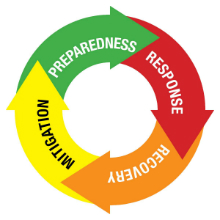
\includegraphics[scale=0.7]{common-emergency.jpg}
\caption{Common Emergency Cycle\cite{CommonEmg}}
\label{fig:emg-cycle}
\end{center}
\end{figure}\par

\section{Theoritical Review}
There are many other research about  service system engineering and disaster management. To build a good service, it is necessary how the plan before, develop and manage the infrastructure development, products and services from Disaster Management. Furthermore, this research will use the framework of IT services to generate Disaster Management based IT services. many problems come since Indonesia Used HFA as Disaster Risk Reduction (DRR) guide. The formation of BNPB (the national agency for disaster management) and Law 24/2007 on Disaster Management have been the key drivers for progress in DRR. However, we have also revealed that local stakeholders are progressing considerably slower and at vastly different rates compared with their national counterpart. An imperative now is to improve the capacity and capability of local actors to manage resilience. \par  
Services are activities that cause a transformation of the state of an entity (people, product, business, and region or nation) by mutually agreed terms between the service provider and the customer. Individual services are relatively simple, although they may require customization and significant backstage support (e.g., database, knowledge management, analysis, forecasting, etc.) to assure quality and timely delivery. Service System Engineering (SSE) has two core concept. Lopez and Pineda (2013) mention two core concept of SSE are service Meta-Model and Service Systems Development Process (SSDP). Service meta-model comprised of nine types of system entities to help business challenge and to create the the service value chain among relevant stakeholders to co-create the value.\par


\section{Research Gap}
The disaster management is research many times, and from the research gives many references too. Although the research issued in social and behaviour issue. Service engineering is research many times too, and one of many paper provides the reference about the many application can be used in implementation of it. The Development of a model to investigate the disaster management system performance on the evacuation operation by employing different city with evacuation strategies. We reported our recent work on two major evacuation strategies, Demand Strategies (DS) and Speed Strategies (SS) which provide significantly improved evacuation results in smart cities settings. The future work will focus on further analysis and validation of additional disaster evacuation strategies.\par

